\section{Techniken}

\subsection{Finden von Hypothesenraum}
\begin{frame}
	\frametitle{Subsumption}
	Finden einer neuen Hypothese einfacher durch Eingrenzung von Suchraum

	Einführung der \textbf{Subsumption}
	\begin{block}{Definition: Subsumption für Literale/Atome}
		Seien $L_1$ und $L_2$ Literale: $L_1 \underbrace{\preceq}_{\text{subsummiert}} L_2$
		wenn eine Substitution $\theta$ existert, sodass:
		\begin{align*}
			 L_1 \theta \subseteq L_2
		\end{align*}
		Beispiel:
		\begin{align*}
			 daughter(X, Y)  \subseteq female(ann), daughter(mary, ann)\\\text{  mit  } \theta = \{X/mary, Y/ann\}
		\end{align*}
	\end{block}
\end{frame}
\begin{frame}
	\frametitle{Subsumption}
	Das gleiche Prozedere für Klauseln:
	\begin{block}{Definition: Subsumption für Klauseln}
		Seien $C_1$ und $C_2$ Literale: $C_1 \underbrace{\preceq}_{\text{subsummiert}} C_2$
		wenn eine Substitution $\theta$ existert, sodass:
		\begin{align*}
			 C_1 \theta \subseteq C_2
		\end{align*}
		Beispiel:
		\begin{gather*}
			 daughter(X, Y) \leftarrow parent(Y,X) \subseteq\\
			 daughter(mary, ann) \leftarrow parent(ann, mary), parent(ann, tom)\\
			 \text{  mit  } \theta = \{X/mary, Y/ann\}
		\end{gather*}
	\end{block}
\end{frame}

\begin{frame}
	\frametitle{Eigenschaften der Subsumption}
	\begin{enumerate}
		\item {
			Wenn $C_1 \preceq C_2$ dann gilt:
			\begin{align*}
				C_1 \vDash C_2
			\end{align*}
		}
		\item{ Die Relation $\leq$ führt ein Gitter (lattice) von reduzierten Klauseln ein
			\begin{figure}[H]
				\begin{center}
					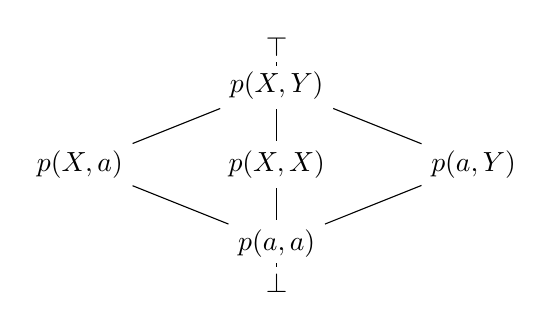
\begin{tikzpicture}
						\node (G) at (1.5,2) {$\top$};
						\node (A) at (1.5,1.5) {$p(X,Y)$};
						\node (B) at (-1,0.5) {$p(X,a)$};
						\node (C) at (1.5,0.5) {$p(X,X)$};
						\node (D) at (4,0.5) {$p(a,Y)$};
						\node (E) at (1.5,-0.5) {$p(a,a)$};
						\node (F) at (1.5,-1) {$\bot$};
			
						\path [-] (A) edge node[left] {} (G);
						\path [-] (A) edge node[left] {} (B);
						\path [-] (A) edge node[left] {} (C);
						\path [-] (A) edge node[left] {} (D);
						\path [-] (B) edge node[left] {} (E);
						\path [-] (C) edge node[left] {} (E);
						\path [-] (D) edge node[left] {} (E);
						\path [-] (F) edge node[left] {} (E);
					\end{tikzpicture}
				\end{center}
				\caption{Example for POSET of atomic formulas}
				\label{fig:poset_atomic}
			\end{figure}
		}
	\end{enumerate}
\end{frame}

\subsection{LGG}
\begin{frame}
	\frametitle{Least general generalization (LGG)}
	 Die \textit{least general generalization} von zwei Klauseln $C_1, C_2$ ist
	 die kleinste obere Schranke von $C_1,C_2$ im Gitter.

	\begin{block}{Erkenntnisse}
			\begin{itemize}
				\item [$\Rightarrow$] Alle Beispiele die $C_1$ abdeckt werden auch von
				allen 'kleineren Klauseln' abgedeckt
				\item[$\Rightarrow$] Wenn $C_1$ ein Beispiel nicht abdeckt,
				dann tut dies auch keine 'kleinere Klausel'
			\end{itemize}
	 \end{block}
\end{frame}

\begin{frame}
\frametitle{LGG - Algorithmus}
	\begin{block}{$lgg$ von Termen}
		\begin{enumerate}
			\item $lgg(t,t) = t$\\
			\item $lgg(f(s_1, \ldots, s_n), f(t_1, \ldots, t_n)) = f(lgg(s_1, t_1), \ldots, lgg(s_n, t_n))$
			\item Sonst: $lgg(t_1, t_2) = v , v$ freie Variable
		\end{enumerate}
	\end{block}
	\begin{block}{$lgg$ von Literalen}
	\begin{enumerate}
		\item $lgg(p(u_1, \ldots, u_n), p(s_1, \ldots, s_n)) = p(lgg(u_1, s_1), \ldots, lgg(u_n, s_n))$\\
		\item Sonst: $lgg(L_1, L_2) = \top$
	\end{enumerate}
	\end{block}
\end{frame}


\subsection{Bottom-up}
\begin{frame}
\frametitle{RLGG - Algorithmus}
\begin{block}{Definition -- Relative least general generalization}
	Gegeben: Hintergrundwissen besteht nur aus \textit{ground literals} (Literale ohne Variablen)
	Sei $K$ die Konjunktion aller Hintergrundliterale und $e_1, e_2$ positive Beispiele
	\begin{align*}
		rlgg(e_1, e_2) = lgg((e_1 \leftarrow K), (e_2 \leftarrow K))
	\end{align*}
\end{block}

Beispiel: Gegebene Familienkonstellation:
\img{family_relation}{}{Familienrelation}{0.4}
\end{frame}


\begin{frame}{Linearity}
\frametitle{RLGG Anschaulich}
	\pgfdeclarelayer{background}
	\pgfsetlayers{background,main}
	\tikzstyle{vertex}=[rectangle,fill=black!25,minimum size=20pt,inner sep=0pt]
	\tikzstyle{selected vertex} = [vertex, fill=red!24]
	\tikzstyle{edge} = [draw,thick,-]
	\tikzstyle{weight} = [font=\small]
	\tikzstyle{selected edge} = [draw,line width=5pt,-,red!50]
	\setbeamercovered{invisible}
	\begin{figure}
		\begin{tikzpicture}[scale=1.0, auto,swap]
		\node[vertex] (a) at (0,0) {$A = e_1 \leftarrow K$};
		\node[vertex] (b) at (2.5,0) {$B = e_2 \leftarrow K$};
		\node[vertex] (c) at (5,0) {$C = e_3 \leftarrow K$};
		\node[vertex] (d) at (7.5,0) {$D = e_4 \leftarrow K$};\pause
		\node[vertex] (e) at (1.25,2) {$C' = lgg(A, B)$};
		\node[vertex] (f) at (6.25,2) {$C''= lgg(C, D)$};\pause
		\node[vertex] (g) at (3.75,4) {$\mathcal{H} = lgg(C', C'')$};
		\begin{pgfonlayer}{background}
			\path<2->[selected edge] (a.center) -- (e.center);
			\path<2->[selected edge] (b.center) -- (e.center);
			\path<2->[selected edge] (c.center) -- (f.center);
			\path<2->[selected edge] (d.center) -- (f.center);
			\path<3->[selected edge] (e.center) -- (g.center);
			\path<3->[selected edge] (f.center) -- (g.center);
		\end{pgfonlayer}
		\end{tikzpicture}
	\end{figure}
\end{frame}

\begin{frame}
\frametitle{RLGG - Algorithmus Erweitert}
Probleme: Große Klauseln bei kleinen Beispielen
Vorheriges Beispiel:
\begin{gather*}
K = p(h,m), p(h,t), p(t,e), P(t,i), f(h), f(m), f(e)\\
rlgg(e_1, e_2) = lgg((e_1 \leftarrow K), (e_2 \leftarrow K))\\
\begin{split}
\underline{d(V_{m,e}, V_{h,t})} \leftarrow &\; p(h,m), p(h,t), p(t,e), p(t,i), f(h), f(m), f(e),\\
&\; p(h, V_{m,t}), \underline{p(V_{h,t}, V_{m,e})}, p(V_{h,t}, V_{m,i}), p(V_{h,t}, V_{t,e}),\\
&\; p(V_{h,t}, V_{t,i}) ,p(t, V_{e,i}), f(V_h, m), f(V_{h,e}), \underline{f(V_{m,e})}
\end{split}
\end{gather*}

Weiteres Probleme:
\begin{itemize}
	\item $K$ bekommen wenn es nicht nur aus \textit{ground literals} besteht (Anhang: Saturierung)
	\item $\mathcal{H}$ kann nicht mehr als \emph{eine} Klausel umfassen
\end{itemize}

\end{frame}

\subsection{Top-down}
\begin{frame}
\frametitle{Top-Down Ansatz}
Idee: Klauseln zu immer weiter spezifizieren

\begin{block}{Der Refinement-Operator $\rho$}
\begin{align*}
	\forall D \in \rho(C). C \preceq D
\end{align*}
\end{block}
\end{frame}

\subsection{Refinement-Operator}
\begin{frame}
\frametitle{Refinement-Operator}
Beispiel für $\rho$:

\begin{figure}[H]
	\begin{center}
		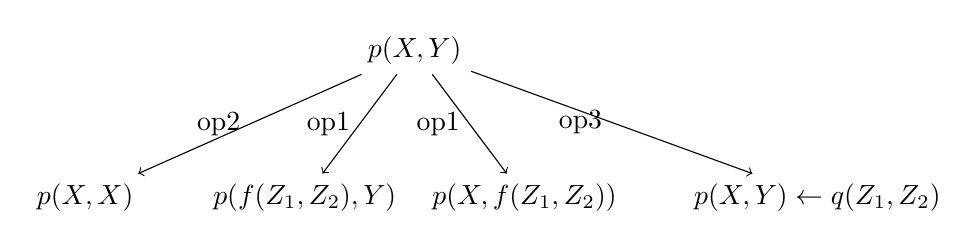
\begin{tikzpicture}[scale=0.93]
			\node (A) at (1.5,1) {$p(X,Y)$};
			\node (B) at (-3,-1) {$p(X,X)$};
			\node (C) at (0,-1) {$p(f(Z_1,Z_2), Y)$};
			\node (D) at (3,-1) {$p(X,f(Z_1,Z_2))$};
			\node (E) at (7,-1) {$p(X,Y) \leftarrow q(Z_1, Z_2)$};

			\path [->] (A) edge node[left] {op2} (B);
			\path [->] (A) edge node[left] {op1} (C);
			\path [->] (A) edge node[left] {op1} (D);
			\path [->] (A) edge node[left] {op3} (E);
		\end{tikzpicture}
	\end{center}
	\caption{Beispiel für refinement operators}
	\label{fig:refinement_operator}
\end{figure}
\end{frame}
